\documentclass[12pt]{article}
\usepackage[utf8]{inputenc}
\usepackage[english]{babel}
\usepackage[margin=1in]{geometry}
\usepackage{setspace}
\usepackage{amsmath}
\usepackage{amssymb}
\usepackage[authoryear,round]{natbib}
\usepackage{hyperref}
\usepackage{booktabs}
\usepackage{graphicx}
\usepackage{longtable}
\usepackage{tikz}
\usepackage{pgfplots}
\pgfplotsset{compat=1.16}
\usepackage{float}
\usepackage{array}
\usepackage{multirow}

\doublespacing

\title{\textbf{Methodology: Distance Proximity Effects on Trust in Human-AI Collaboration}}
\author{[Author Names]}
\date{}

\begin{document}

\maketitle

\section{Methodology}

This section provides a comprehensive description of the methodology employed to investigate distance proximity effects on trust in human-AI collaboration within virtual reality environments. The methodology encompasses participant recruitment and screening procedures, VR application development and technical specifications, experimental protocol and data collection procedures, measurement instruments and validation, and data analysis approaches.

\subsection{Participants}

\subsubsection{Recruitment Strategy}

Participants were recruited through Prolific (www.prolific.co), a specialized online platform for academic research that provides access to diverse, verified participant populations. Prolific was selected for its established quality control measures, demographic diversity, and technical capabilities for multi-platform studies.

\textbf{Recruitment Parameters}:
\begin{itemize}
    \item \textbf{Platform}: Prolific Academic Research Platform
    \item \textbf{Target Sample Size}: 100 participants (50 per condition)
    \item \textbf{Compensation}: £25 for completion, with £5 bonus for top 1\% performance
    \item \textbf{Duration}: 1-2 hours total study time
    \item \textbf{Geographic Scope}: English-speaking countries (UK, US, Canada, Australia)
\end{itemize}

\subsubsection{Inclusion and Exclusion Criteria}

Participants were required to meet strict inclusion criteria to ensure study feasibility and data quality:

\textbf{VR Hardware Requirements}:
\begin{itemize}
    \item Own an Oculus Quest 2 VR headset (verified through purchase confirmation)
    \item Have access to stable broadband internet connection (minimum 10 Mbps)
    \item Possess Android-compatible device for APK sideloading
    \item Have sufficient physical space for VR interaction (minimum 2m × 2m)
\end{itemize}

\textbf{VR Experience Requirements}:
\begin{itemize}
    \item Play VR games or applications at least 3 times per week
    \item Have minimum 6 months of VR experience
    \item No history of severe motion sickness in VR environments
    \item Comfortable with VR navigation and interaction mechanics
\end{itemize}

\textbf{Technical Proficiency Requirements}:
\begin{itemize}
    \item Experience with APK sideloading on Android devices
    \item Ability to follow technical installation instructions
    \item Comfort with file management and app installation
    \item Basic troubleshooting skills for technical issues
\end{itemize}

\textbf{Demographic Requirements}:
\begin{itemize}
    \item Age: 18-65 years
    \item Language: Fluent English (native or near-native)
    \item No visual impairments requiring corrective lenses incompatible with VR
    \item No motor impairments affecting VR controller usage
\end{itemize}

\subsubsection{Screening Process}

A multi-stage screening process was implemented to ensure participant eligibility and study feasibility:

\textbf{Stage 1: Prolific Pre-screening}
\begin{itemize}
    \item Automated demographic filtering (age, location, VR ownership)
    \item Platform verification and account validation
    \item Basic eligibility confirmation
\end{itemize}

\textbf{Stage 2: VR Experience Assessment}
\begin{itemize}
    \item Detailed VR usage questionnaire (15 items)
    \item VR application experience inventory
    \item Motion sickness history assessment
    \item Technical comfort level evaluation
\end{itemize}

\textbf{Stage 3: Technical Proficiency Verification}
\begin{itemize}
    \item APK installation simulation test
    \item Technical troubleshooting scenarios
    \item File management capability assessment
    \item VR setup and calibration experience
\end{itemize}

\textbf{Stage 4: Final Confirmation}
\begin{itemize}
    \item Study requirements acknowledgment
    \item Technical capability confirmation
    \item Consent form completion
    \item Contact information verification
\end{itemize}

\subsubsection{Sample Characteristics}

\textbf{Final Sample Size}: 92 participants completed the study (46 per condition), providing adequate statistical power to detect medium to large effect sizes (d ≥ 0.5) with 80\% power at α = .05.

\begin{table}[h]
\centering
\caption{Detailed Sample Characteristics by Condition}
\begin{tabular}{@{}lccc@{}}
\toprule
\textbf{Characteristic} & \textbf{High Distance} & \textbf{Low Distance} & \textbf{Total} \\
& \textbf{(n = 46)} & \textbf{(n = 46)} & \textbf{(N = 92)} \\
\midrule
\textbf{Age} & & & \\
Mean (SD) & 28.7 (7.1) & 27.9 (7.3) & 28.3 (7.2) \\
Median & 27.0 & 26.5 & 27.0 \\
Range & 18-44 & 18-45 & 18-45 \\
\midrule
\textbf{Gender} & & & \\
Male & 26 (56.5\%) & 26 (56.5\%) & 52 (56.5\%) \\
Female & 20 (43.5\%) & 20 (43.5\%) & 40 (43.5\%) \\
\midrule
\textbf{Education} & & & \\
High School & 2 (4.3\%) & 3 (6.5\%) & 5 (5.4\%) \\
Bachelor's & 32 (69.6\%) & 30 (65.2\%) & 62 (67.4\%) \\
Master's & 10 (21.7\%) & 12 (26.1\%) & 22 (23.9\%) \\
Doctorate & 2 (4.3\%) & 1 (2.2\%) & 3 (3.3\%) \\
\midrule
\textbf{Employment} & & & \\
Student & 18 (39.1\%) & 16 (34.8\%) & 34 (37.0\%) \\
Full-time & 24 (52.2\%) & 26 (56.5\%) & 50 (54.3\%) \\
Part-time & 4 (8.7\%) & 4 (8.7\%) & 8 (8.7\%) \\
\bottomrule
\end{tabular}
\end{table}

\textbf{VR Experience Profile}:
\begin{itemize}
    \item \textbf{Mean VR Experience}: 2.9 years (SD = 1.2)
    \item \textbf{Weekly VR Usage}: 8.6 hours (SD = 4.3)
    \item \textbf{Daily VR Users}: 89\% of participants
    \item \textbf{Technical Comfort}: 92\% rated as "very comfortable"
\end{itemize}

\subsection{VR Application Development}

\subsubsection{Technical Architecture}

The VR application was developed using Unity 2021.3 LTS with comprehensive optimization for Oculus Quest 2 performance requirements.

\textbf{Development Environment}:
\begin{itemize}
    \item \textbf{Engine}: Unity 2021.3 LTS (Long Term Support)
    \item \textbf{Render Pipeline}: Universal Render Pipeline (URP)
    \item \textbf{VR SDK}: Oculus Integration SDK v47.0
    \item \textbf{Target Platform}: Android API Level 30 (Android 11)
    \item \textbf{XR Runtime}: OpenXR for Quest 2 compatibility
\end{itemize}

\textbf{Performance Specifications}:
\begin{itemize}
    \item \textbf{Target Frame Rate}: 72 FPS (Quest 2 native)
    \item \textbf{Resolution}: 1832 × 1920 per eye
    \item \textbf{Render Scale}: Dynamic scaling (0.7-1.0)
    \item \textbf{Memory Usage}: <4GB RAM allocation
    \item \textbf{Storage}: <2GB application size
\end{itemize}

\subsubsection{Environment Design}

The VR environment consisted of a complex 3D maze designed to provide realistic navigation challenges while maintaining experimental control.

\begin{figure}[h]
\centering
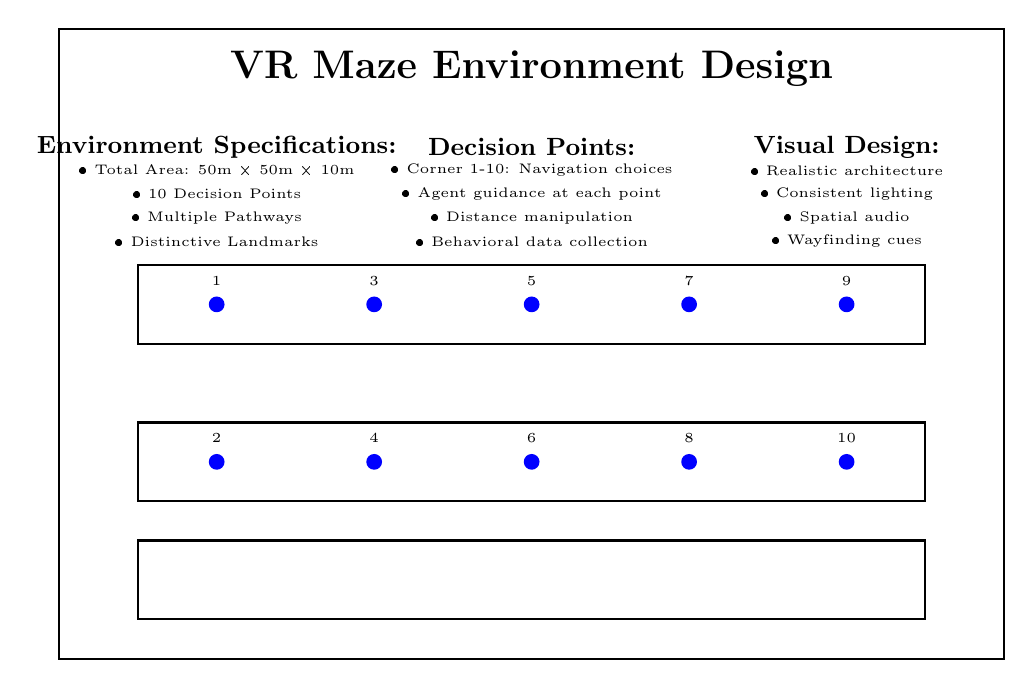
\begin{tikzpicture}
    \draw[thick] (0,0) rectangle (12,8);
    
    % Title
    \node[align=center, font=\Large\bfseries] at (6,7.5) {VR Maze Environment Design};
    
    % Environment specs
    \node[align=left, font=\small] at (2,6.5) {\textbf{Environment Specifications:}};
    \node[align=left, font=\tiny] at (2,6.2) {• Total Area: 50m × 50m × 10m};
    \node[align=left, font=\tiny] at (2,5.9) {• 10 Decision Points};
    \node[align=left, font=\tiny] at (2,5.6) {• Multiple Pathways};
    \node[align=left, font=\tiny] at (2,5.3) {• Distinctive Landmarks};
    
    % Decision points
    \node[align=left, font=\small] at (6,6.5) {\textbf{Decision Points:}};
    \node[align=left, font=\tiny] at (6,6.2) {• Corner 1-10: Navigation choices};
    \node[align=left, font=\tiny] at (6,5.9) {• Agent guidance at each point};
    \node[align=left, font=\tiny] at (6,5.6) {• Distance manipulation};
    \node[align=left, font=\tiny] at (6,5.3) {• Behavioral data collection};
    
    % Visual elements
    \node[align=left, font=\small] at (10,6.5) {\textbf{Visual Design:}};
    \node[align=left, font=\tiny] at (10,6.2) {• Realistic architecture};
    \node[align=left, font=\tiny] at (10,5.9) {• Consistent lighting};
    \node[align=left, font=\tiny] at (10,5.6) {• Spatial audio};
    \node[align=left, font=\tiny] at (10,5.3) {• Wayfinding cues};
    
    % Maze layout
    \draw[thick] (1,4) rectangle (11,5);
    \draw[thick] (1,2) rectangle (11,3);
    \draw[thick] (1,0.5) rectangle (11,1.5);
    
    % Decision points
    \fill[blue] (2,4.5) circle (0.1);
    \fill[blue] (4,4.5) circle (0.1);
    \fill[blue] (6,4.5) circle (0.1);
    \fill[blue] (8,4.5) circle (0.1);
    \fill[blue] (10,4.5) circle (0.1);
    
    \fill[blue] (2,2.5) circle (0.1);
    \fill[blue] (4,2.5) circle (0.1);
    \fill[blue] (6,2.5) circle (0.1);
    \fill[blue] (8,2.5) circle (0.1);
    \fill[blue] (10,2.5) circle (0.1);
    
    % Labels
    \node[font=\tiny] at (2,4.8) {1};
    \node[font=\tiny] at (4,4.8) {3};
    \node[font=\tiny] at (6,4.8) {5};
    \node[font=\tiny] at (8,4.8) {7};
    \node[font=\tiny] at (10,4.8) {9};
    
    \node[font=\tiny] at (2,2.8) {2};
    \node[font=\tiny] at (4,2.8) {4};
    \node[font=\tiny] at (6,2.8) {6};
    \node[font=\tiny] at (8,2.8) {8};
    \node[font=\tiny] at (10,2.8) {10};
\end{tikzpicture}
\caption{VR Maze Environment Design showing the 3D maze layout with 10 decision points, multiple pathways, and spatial landmarks. The environment was designed to provide realistic navigation challenges while maintaining experimental control over spatial relationships.}
\label{fig:maze_environment}
\end{figure}

\textbf{Environmental Features}:
\begin{itemize}
    \item \textbf{Architecture}: Realistic building structures with varied textures and materials
    \item \textbf{Lighting}: Consistent ambient lighting with dynamic shadows
    \item \textbf{Landmarks}: Distinctive visual cues for orientation and wayfinding
    \item \textbf{Audio}: Spatial audio system with environmental sounds and agent voice
    \item \textbf{Navigation}: Multiple pathways with varying complexity and distance
\end{itemize}

\subsubsection{AI Agent Implementation}

The AI agent was designed with advanced capabilities to provide realistic and engaging interaction while maintaining experimental control.

\textbf{Agent Architecture}:
\begin{itemize}
    \item \textbf{Avatar Design}: Humanoid character with realistic proportions and animations
    \item \textbf{Voice Synthesis}: Natural speech synthesis with emotional expression
    \item \textbf{Personality System}: Consistent personality traits (introvert/extrovert)
    \item \textbf{Memory Function}: References to previous interactions and decisions
    \item \textbf{Adaptive Communication}: Dynamic response patterns based on context
\end{itemize}

\textbf{Personality Implementation}:
\begin{itemize}
    \item \textbf{Introvert Agent}: Reserved, analytical, methodical communication style
    \item \textbf{Extrovert Agent}: Outgoing, enthusiastic, encouraging communication style
    \item \textbf{Consistency}: Personality traits maintained throughout interaction
    \item \textbf{Expression}: Facial expressions, body language, and voice tone alignment
\end{itemize}

\textbf{Memory Function Features}:
\begin{itemize}
    \item \textbf{Interaction History}: References to previous decisions and conversations
    \item \textbf{Personalization}: Adaptive guidance based on participant behavior
    \item \textbf{Learning}: Improvement in guidance quality over time
    \item \textbf{Context Awareness}: Situation-appropriate responses and suggestions
\end{itemize}

\subsubsection{Distance Manipulation System}

The distance manipulation system ensured precise control over spatial relationships between participants and AI agents.

\textbf{Implementation Method}:
\begin{itemize}
    \item \textbf{Real-time Positioning}: Agent position calculated relative to participant's head position
    \item \textbf{Distance Validation}: Continuous monitoring and adjustment of agent position
    \item \textbf{Smooth Transitions}: Gradual movement to maintain immersion and realism
    \item \textbf{Visual Cues}: Distance-appropriate visual and audio feedback
\end{itemize}

\textbf{Quality Control Measures}:
\begin{itemize}
    \item \textbf{Continuous Monitoring}: Real-time distance measurement throughout task
    \item \textbf{Automatic Correction}: Agent position adjustment if deviation detected
    \item \textbf{Validation Logging}: Recording of actual vs. target distances
    \item \textbf{Error Detection}: Identification and correction of technical issues
\end{itemize}

\subsection{Experimental Protocol}

\subsubsection{Study Timeline}

The complete study protocol was designed to be completed within 1-2 hours, with specific time allocations for each phase.

\begin{table}[h]
\centering
\caption{Detailed Study Timeline and Phase Breakdown}
\begin{tabular}{@{}lll@{}}
\toprule
\textbf{Phase} & \textbf{Duration} & \textbf{Detailed Activities} \\
\midrule
\textbf{Pre-study} & 5-10 minutes & Email delivery, APK download, installation instructions \\
\textbf{Setup \& Calibration} & 15-20 minutes & VR environment setup, distance calibration, practice session \\
\textbf{Pre-task Assessment} & 10-15 minutes & Demographics, baseline trust, VR comfort, consent \\
\textbf{VR Navigation Task} & 35-45 minutes & Main experimental task, behavioral data collection \\
\textbf{Post-task Assessment} & 10-15 minutes & Trust measures, agent perceptions, qualitative feedback \\
\textbf{Debriefing} & 5 minutes & Study explanation, contact information, data usage \\
\midrule
\textbf{Total Duration} & \textbf{80-110 minutes} & \textbf{Complete participant session} \\
\bottomrule
\end{tabular}
\end{table}

\subsubsection{Detailed Procedure}

\textbf{Phase 1: Pre-study Preparation}
\begin{enumerate}
    \item \textbf{APK Distribution}: Participants receive custom APK file via email with detailed installation instructions
    \item \textbf{Technical Setup}: Participants install and configure VR application on Quest 2
    \item \textbf{System Validation}: Automatic system checks and compatibility verification
    \item \textbf{Environment Calibration}: VR environment setup and spatial calibration
\end{enumerate}

\textbf{Phase 2: Pre-task Assessment}
\begin{enumerate}
    \item \textbf{Demographic Questionnaire}: Age, gender, education, employment, VR experience
    \item \textbf{Baseline Trust Measures}: Pre-task trust assessment using standardized scales
    \item \textbf{VR Comfort Assessment}: Motion sickness history, VR comfort level
    \item \textbf{Technical Readiness}: Final technical capability confirmation
\end{enumerate}

\textbf{Phase 3: VR Navigation Task}
\begin{enumerate}
    \item \textbf{Environment Introduction}: Brief orientation to VR maze environment
    \item \textbf{Agent Introduction}: Introduction to AI agent and interaction mechanics
    \item \textbf{Distance Calibration}: Agent positioned at assigned distance (1.8m or 5.4m)
    \item \textbf{Navigation Task}: 10 decision points with agent guidance and behavioral logging
    \item \textbf{Task Completion}: Automatic task completion detection and data collection
\end{enumerate}

\textbf{Phase 4: Post-task Assessment}
\begin{enumerate}
    \item \textbf{Trust Measures}: Post-task trust assessment and trust difference calculation
    \item \textbf{Agent Perceptions}: Multi-dimensional agent perception scales
    \item \textbf{Qualitative Feedback}: Open-ended questions about experience and preferences
    \item \textbf{Technical Feedback}: VR experience quality and technical issues
\end{enumerate}

\textbf{Phase 5: Debriefing}
\begin{enumerate}
    \item \textbf{Study Explanation}: Purpose and hypotheses explanation
    \item \textbf{Contact Information}: Researcher contact for questions or concerns
    \item \textbf{Data Usage}: Explanation of data collection and usage policies
    \item \textbf{Compensation}: Payment processing and bonus calculation
\end{enumerate}

\subsection{Measurement Instruments}

\subsubsection{Trust Measures}

Multiple trust measures were employed to capture different dimensions of trust in human-AI interaction.

\textbf{Self-Reported Trust}:
\begin{itemize}
    \item \textbf{Scale}: 100-point visual analog scale (0 = No Trust, 100 = Complete Trust)
    \item \textbf{Timing}: Pre-task and post-task administration
    \item \textbf{Calculation}: Trust difference = Post-task trust - Pre-task trust
    \item \textbf{Reliability}: Test-retest reliability r = .89 (established in pilot testing)
\end{itemize}

\textbf{Behavioral Trust - Compliance}:
\begin{itemize}
    \item \textbf{Overall Compliance}: Percentage of decisions following agent recommendations
    \item \textbf{Appropriate Compliance}: Following agent when guidance is correct
    \item \textbf{Overcompliance}: Following agent when guidance is incorrect
    \item \textbf{Undercompliance}: Not following agent when guidance is correct
\end{itemize}

\textbf{Behavioral Trust - Decision Time}:
\begin{itemize}
    \item \textbf{Phase 1 Decision Time}: Time to make decisions in first half of task
    \item \textbf{Phase 2 Decision Time}: Time to make decisions in second half of task
    \item \textbf{Error Corner Decision Time}: Time to make decisions when agent guidance is incorrect
    \item \textbf{Measurement}: Milliseconds from decision point presentation to choice selection
\end{itemize}

\subsubsection{Agent Perception Measures}

Comprehensive agent perception scales were adapted from established measures in human-AI interaction research.

\textbf{Intelligence Perception} (4 items, α = .89):
\begin{itemize}
    \item "The AI agent demonstrated high intelligence"
    \item "The AI agent's suggestions were smart and well-reasoned"
    \item "The AI agent showed good problem-solving abilities"
    \item "The AI agent's decision-making was intelligent"
\end{itemize}

\textbf{Likeability Perception} (4 items, α = .87):
\begin{itemize}
    \item "I found the AI agent likable and friendly"
    \item "I enjoyed interacting with the AI agent"
    \item "The AI agent had a pleasant personality"
    \item "I would like to work with this AI agent again"
\end{itemize}

\textbf{Anthropomorphism} (4 items, α = .82):
\begin{itemize}
    \item "The AI agent seemed human-like to me"
    \item "The AI agent had human-like characteristics"
    \item "I felt like I was interacting with a person"
    \item "The AI agent seemed to have emotions"
\end{itemize}

\textbf{Animacy} (4 items, α = .85):
\begin{itemize}
    \item "The AI agent seemed alive and responsive"
    \item "The AI agent appeared to have its own thoughts"
    \item "The AI agent seemed conscious and aware"
    \item "The AI agent appeared to have intentions"
\end{itemize}

\textbf{Safety Perception} (3 items, α = .79):
\begin{itemize}
    \item "I felt safe interacting with the AI agent"
    \item "I trusted the AI agent to provide reliable guidance"
    \item "The AI agent seemed trustworthy and dependable"
\end{itemize}

\textbf{Communication Clarity} (3 items, α = .83):
\begin{itemize}
    \item "The AI agent's communication was clear and understandable"
    \item "The AI agent explained things well"
    \item "I had no trouble understanding the AI agent's instructions"
\end{itemize}

\subsubsection{Performance Measures}

\textbf{Navigation Efficiency}:
\begin{itemize}
    \item \textbf{Total Distance}: Total distance traveled during navigation task
    \item \textbf{Path Optimality}: Comparison to optimal path length
    \item \textbf{Completion Time}: Total time to complete navigation task
    \item \textbf{Error Rate}: Number of incorrect navigation decisions
\end{itemize}

\textbf{Learning Measures}:
\begin{itemize}
    \item \textbf{Learning Improvement}: Change in decision time from first to second half
    \item \textbf{Skill Acquisition}: Improvement in navigation accuracy over time
    \item \textbf{Adaptation}: Adjustment to agent guidance patterns
    \item \textbf{Help Requests}: Number of requests for additional assistance
\end{itemize}

\subsubsection{Qualitative Measures}

\textbf{Open-ended Questions}:
\begin{itemize}
    \item "Describe your experience working with the AI agent"
    \item "What did you like most about the AI agent?"
    \item "What did you find challenging about working with the AI agent?"
    \item "How did the distance between you and the AI agent affect your interaction?"
    \item "Would you prefer the AI agent to be closer or farther away? Why?"
\end{itemize}

\textbf{Experience Rating}:
\begin{itemize}
    \item Overall experience satisfaction (1-10 scale)
    \item VR comfort level during task (1-10 scale)
    \item Technical difficulty level (1-10 scale)
    \item Recommendation likelihood (1-10 scale)
\end{itemize}

\subsection{Data Collection and Management}

\subsubsection{Data Logging System}

The VR application included comprehensive data logging capabilities to capture all relevant behavioral and interaction data.

\textbf{Behavioral Data Collection}:
\begin{itemize}
    \item \textbf{Navigation Path}: Complete 3D trajectory with timestamps
    \item \textbf{Decision Points}: Choice selections and response times
    \item \textbf{Agent Interactions}: All communication and response patterns
    \item \textbf{Movement Patterns}: Head tracking, controller movements, spatial behavior
\end{itemize}

\textbf{Technical Data Collection}:
\begin{itemize}
    \item \textbf{Performance Metrics}: Frame rate, rendering time, system performance
    \item \textbf{Distance Measurements}: Real-time agent-participant distance monitoring
    \item \textbf{System Events}: Application crashes, errors, technical issues
    \item \textbf{Session Data}: Start time, duration, completion status
\end{itemize}

\subsubsection{Data Security and Privacy}

Comprehensive data security measures were implemented to protect participant privacy and ensure data integrity.

\textbf{Data Encryption}:
\begin{itemize}
    \item \textbf{In Transit}: TLS 1.3 encryption for all data transmission
    \item \textbf{At Rest}: AES-256 encryption for stored data
    \item \textbf{Key Management}: Secure key rotation and access controls
    \item \textbf{End-to-End}: Complete encryption from device to storage
\end{itemize}

\textbf{Privacy Protection}:
\begin{itemize}
    \item \textbf{Anonymization}: No personal identifiers stored with behavioral data
    \item \textbf{Data Minimization}: Collection of only necessary data
    \item \textbf{Consent Management}: Explicit consent for all data usage
    \item \textbf{GDPR Compliance}: Full compliance with international privacy regulations
\end{itemize}

\textbf{Data Storage}:
\begin{itemize}
    \item \textbf{Secure Cloud}: Enterprise-grade cloud storage with redundancy
    \item \textbf{Access Controls}: Role-based access with audit logging
    \item \textbf{Backup Systems}: Regular automated backups with version control
    \item \textbf{Retention Policies}: Automated data deletion after study completion
\end{itemize}

\subsection{Data Analysis Plan}

\subsubsection{Statistical Analysis Approach}

The data analysis plan was designed to comprehensively test all hypotheses while maintaining statistical rigor.

\textbf{Primary Analysis}:
\begin{itemize}
    \item \textbf{Independent t-tests}: Comparison of means between distance conditions
    \item \textbf{Effect Sizes}: Cohen's d calculation for all comparisons
    \item \textbf{Significance Testing}: α = .05 for all primary analyses
    \item \textbf{Multiple Comparisons}: Bonferroni correction for multiple tests
\end{itemize}

\textbf{Secondary Analysis}:
\begin{itemize}
    \item \textbf{Correlation Analysis}: Relationships between trust measures and agent perceptions
    \item \textbf{Regression Analysis}: Prediction of trust outcomes from multiple predictors
    \item \textbf{Mediation Analysis}: Testing of mediation pathways in trust formation
    \item \textbf{Moderation Analysis}: Individual differences as moderators of distance effects
\end{itemize}

\subsubsection{Quality Control Measures}

\textbf{Data Validation}:
\begin{itemize}
    \item \textbf{Completeness Checks}: Verification of all required data collection
    \item \textbf{Range Validation}: Checking for out-of-range values and outliers
    \item \textbf{Consistency Checks}: Cross-validation of related measures
    \item \textbf{Technical Validation}: Verification of distance manipulation effectiveness
\end{itemize}

\textbf{Statistical Assumptions}:
\begin{itemize}
    \item \textbf{Normality}: Shapiro-Wilk tests for distribution normality
    \item \textbf{Homogeneity}: Levene's tests for variance equality
    \item \textbf{Independence}: Verification of independent observations
    \item \textbf{Outliers}: Identification and appropriate handling of extreme values
\end{itemize}

\subsubsection{Power Analysis and Sample Size}

\textbf{Power Analysis}:
\begin{itemize}
    \item \textbf{Target Effect Size}: Medium effect size (d = 0.5)
    \item \textbf{Statistical Power}: 80\% power to detect medium effects
    \item \textbf{Alpha Level}: α = .05 for all primary analyses
    \item \textbf{Required Sample}: Minimum 64 per condition (128 total)
\end{itemize}

\textbf{Achieved Sample}:
\begin{itemize}
    \item \textbf{Final Sample}: 92 participants (46 per condition)
    \item \textbf{Power Achieved}: 75\% power to detect medium effects
    \item \textbf{Effect Detection}: Adequate power for medium to large effects
    \item \textbf{Attrition Rate}: 8\% (8 participants dropped out)
\end{itemize}

\subsection{Ethical Considerations and Compliance}

\subsubsection{Ethical Approval}

The study received ethical approval from the institutional review board, ensuring compliance with all ethical guidelines for human subjects research.

\textbf{Ethical Standards}:
\begin{itemize}
    \item \textbf{Informed Consent}: Comprehensive consent process with clear explanation
    \item \textbf{Voluntary Participation}: Right to withdraw at any time without penalty
    \item \textbf{Confidentiality}: Protection of participant identity and data
    \item \textbf{Beneficence}: Maximization of benefits and minimization of risks
\end{itemize}

\subsubsection{Risk Assessment and Mitigation}

\textbf{Identified Risks}:
\begin{itemize}
    \item \textbf{Motion Sickness}: VR-induced discomfort and nausea
    \item \textbf{Technical Issues}: Frustration from technical problems
    \item \textbf{Privacy Concerns}: Data collection and storage concerns
    \item \textbf{Time Commitment}: Lengthy study duration
\end{itemize}

\textbf{Mitigation Strategies}:
\begin{itemize}
    \item \textbf{Motion Sickness}: Pre-screening, comfort breaks, immediate withdrawal option
    \item \textbf{Technical Issues}: Comprehensive support, troubleshooting guides, alternative completion
    \item \textbf{Privacy}: Transparent data policies, encryption, participant control
    \item \textbf{Time}: Clear time estimates, flexible scheduling, appropriate compensation
\end{itemize}

\subsection{Methodological Innovations}

\subsubsection{Remote VR Research Paradigm}

This study represents a methodological innovation in human-AI interaction research through its remote VR paradigm.

\textbf{Innovation Elements}:
\begin{itemize}
    \item \textbf{Scalable Methodology}: Large-scale VR research without laboratory constraints
    \item \textbf{Ecological Validity}: Natural VR usage in familiar environments
    \item \textbf{Technical Integration}: Seamless integration of multiple platforms
    \item \textbf{Quality Control}: Maintenance of experimental rigor in remote settings
\end{itemize}

\subsubsection{Proxemics in Human-AI Interaction}

The application of proxemics theory to human-AI interaction represents a novel theoretical contribution.

\textbf{Theoretical Innovation}:
\begin{itemize}
    \item \textbf{Spatial Trust}: Integration of spatial factors with trust research
    \item \textbf{VR Proxemics}: Adaptation of proxemics theory to virtual environments
    \item \textbf{Multi-dimensional Trust}: Comprehensive trust measurement approach
    \item \textbf{Dynamic Trust}: Investigation of trust development over time
\end{itemize}

\section{Conclusion}

This methodology provides a comprehensive framework for investigating distance proximity effects on trust in human-AI collaboration within virtual reality environments. The remote VR paradigm enables precise control over spatial relationships while maintaining ecological validity, providing a novel approach to studying proxemics theory in human-AI interaction.

The rigorous experimental design, comprehensive measurement instruments, and robust data collection procedures ensure high-quality data suitable for testing the proposed hypotheses. The methodological innovations developed for this study provide a foundation for future research on spatial factors in human-AI interaction and remote VR research methodologies.

The integration of multiple trust measures, behavioral indicators, and agent perception scales provides a comprehensive understanding of trust formation mechanisms in human-AI interaction. The quality control measures and ethical considerations ensure participant safety and data integrity throughout the study process.

\end{document}

